\documentclass[oneside]{mgr}

\usepackage{polski}      
\usepackage[utf8]{inputenc}
\usepackage[T1]{fontenc} 
\usepackage{indentfirst}
\usepackage{textcomp}
\usepackage{gensymb}
\usepackage{color}
\usepackage[table]{xcolor}
\usepackage{multirow}
\usepackage{multicol}
\usepackage{ltablex}

%pakiety do grafiki
\usepackage{graphicx}
\usepackage{subfigure}
\usepackage{psfrag}


\usepackage{amsmath}
\usepackage{amsfonts}

\usepackage{supertabular}
\usepackage{array}
\usepackage{tabularx}
\usepackage{hhline}
\usepackage{showlabels}
\usepackage{gensymb}

%definicje własnych poleceń
\newcommand{\R}{I\!\!R} %symbol liczb rzeczywistych, działa tylko w
                        %trybie matematycznym
\newtheorem{theorem}{Twierdzenie}[section] %nowe otoczenie do
                                           %składania twierdzeń
\title{Badanie pracy wentylatorowego układu chłodzenia z ogniwami Peltiera}
\engtitle{Control of the cooling system with Peltier module}
\author{Piotr Bogaczyk}
\supervisor{dr inż. Jacek Jagodziński W-4/K-8}
\field{Automatyka i Robotyka (AIR)}
\specialisation{Systemy informatyczne w automatyce (ASI)}

\begin{document}
\maketitle
\tableofcontents

\chapter{Wstęp}
Tematem niniejszej pracy jest projekt układu dla badania ogniwa Peltiera które zostało wykorzystane do regulacji temperatury w komorze chłodniczej. Praca składa się z czterech głównych rozdziałów. Pierwszy z nich opisuje podstawowe prawa i zasady termoelektryczne takie jak efekt Seebecka, efekt Peltiera oraz efekt Thomsona. Rozdział drugi zawiera opis realizacji urządzenia badawczego w skład rozdziału wchodzi opis realizacji układu chłodniczego z wykorzystaniem ogniwa Peltiera. identyfikacyjnej zawierającej opis wykonanych badań w celu pozwalających na identyfikacje obiektu oraz opisu zaimplementowanych sposobów regulacji temperatury w komorze chłodniczej wraz z ich porównaniem. Dodatkowo w pracy zostały zawarte schematy elektryczne wykorzystanych urządzeń elektrycznych wykonane przy pomocy programu Eplan.

\section{Cel i zakres pracy}

Celem pracy jest zaprojektowanie, budowa i wysterowanie komory termicznej wykorzystującej ogniwo Peltiera jako pompę ciepła.

W pracy została opisana zasada działania oraz budowa modułu Peltiera. Opisano również podstawowe zjawiska termoelektryczne które towarzyszą zmianą temperatury w badanych ogniwach termoelektrycznych.

Został zbudowany obiekt badawczy pozwalający na grzanie lub chłodzenie przestrzeni wewnątrz kasety wykonanej z szkła akrylowego. Efekty działania urządzenia badane są przy wykorzystaniu trzech czujników temperatury typu PT0-10. Czujniki pozwalają one na pomiar temperatury ciepłej i chłodnej strony ogniwa Peltiera oraz pomiar temperatury bezpośrednio wewnątrz zbudowanej komory termicznej. Transmisja ciepła pomiędzy otoczeniem a modułem Peltiera zostało usprawnione przez wykorzystane w projekcie radiatory wspomagane wentylatorami. Dodatkowo wewnątrz komory zostały zamontowane cztery rezystory wysokich mocy. Rezystory zostały zastosowane w celu wprowadzania do układu zakłóceń.

W celu badania, regulacji i wysterowania zbudowanego układu zastosowany został sterownik serii: LOGO!8 marki Siemens. Sterownik pozwala na płynną regulację temperatury wewnątrz komory termicznej. Regulacji temperatury dokonuje się na podstawie odczytu danych z trzech czujników temperatury wykorzystanych w projekcie. W pracy zostały przedstawione i przeanalizowane trzy typy regulacji: krokowa, typu PI oraz predykcyjna.

\section{Założenia projektowe}
Praca zakłada stworzenie układu pozwalającego na płynną regulację temperatury w komorze termicznej z wykorzystaniem sterownika LOGO!8. W pracy założono ,że temperatura na zewnątrz stacji jest stała i niezmienna w czasie.

Sygnały pomiarowe oraz sterujące są przekazywane do i z sterownika za pomocą przewodów poprowadzonych w zamaskowanych szynach. Projekt zakłada brak zakłóceń transmisji sygnałów.

Praca zawiera schematy elektryczne które zostały wykonane za pomocą programu EPLAN w standardzie jednokreskowym. Wszystkie schematy zostały wykonane zgodnie z praktyką inżynierską i zawarte w załączniku numer 1: „Schematy elektryczne”.

\chapter{Teoria chłodnictwa termoelektrycznego}
Istotą modułów Peltiera są zmiany temperatury które zachodzą na złączach półprzewodnikowych (n-p lub p-n) pod wpływem przepływu przez nie prądu elektrycznego. Takie zmiany temperatury znajdują szerokie zastosowanie w chłodnictwie. Zastosowanie ogniw Peltiera w chłodnictwie pozwala na wysoce bezawaryjną pracę chłodziarki w różnych orientacjach. 
Ponieważ napięcie elektryczne jest łatwe do kontrolowania i może być dokładnie zmierzone, urządzenia wykorzystujące efekt termoelektryczny umożliwiają bardzo precyzyjną regulację temperatury i automatyzację procesów chłodzenia i ogrzewania. W zależności od kierunku transformacji efekty termoelektryczne dzielą się na: efekt Seebecka, Peltiera i Thomsona.

\section{Efekt Seebecka}
Efekt Seebecka polega na powstawaniu siły termoelektrycznej w otwartym obwodzie złożonym z dwóch różnych półprzewodników jeżeli ich spoiny są utrzymywane w różnych temperaturach. Przy zamknięciu obwodu następuje przepływ prądu który ściśle zależy od różnicy temperatur półprzewodników oraz materiałów z których są wykonane. Obwód taki nazywany jest termoelementem w technice chłodniczej oraz termoparą w technice cieplnej[1].
\begin{eqnarray}
    e_{AB}(T) \approx U_0 + \alpha \cdot T\\
    e_{BA}(T) \approx -U_0 + -\alpha \cdot T_0 \nonumber
\end{eqnarray}
gdzie: \\
$U_0$ napięcie kontaktowe \\
$T$,$T_0$ – temperatura złączy materiałów $A$ i $B$ \\
$\alpha$ - współczynnik Seebecka obwodu \\

W przewodnikach typu "p-n" występują dwa typy przewodności. Odpowiednio przewodność elektronowa w której nośnikami ładunków są elektrony i dziurowa w której nośnikami są dodatnio naładowane dziury. Jeśli moduł składa się z półprzewodników tego samego typu, w takim wypadku siły termoelektryczne które występują w obwodzie posiadają przeciwne zwroty[1]:
\begin{eqnarray}
    a_p=a_{p1}-a_{p2}, \qquad a_n=a_{n1}-a_{n2}
\end{eqnarray}
Przy różnych rodzajach przewodności spoin siły termoelektromotoryczne sumują się:
\begin{eqnarray}
    \Bar{\alpha}=|\alpha_p|+|\alpha_n|
\end{eqnarray}

W konsekwencji termoelementy wykonuje się głównie z materiałów o różnej przewodności: elektronowej i dziurowej. Każdy zestaw p-n składa się z dwóch gałęzi: typu "n" oraz "p" nazywanych również półelementami. Półelementy typu "p" oraz "n" są połączone ze sobą tak zwanymi mostkami do których są przymocowane przy pomocy lutowania miękiego lub specjalistycznego kleju przewodzącego. Mostki łączące zwykle wykonuje się z miedzi[1] (rys. 2.1)

Takie szeregowe naprzemienne połączenie par przewodników "p" i "n" stanowi siłę termoelektromotoryczną modułu. Wyznacza się ją z zależności[1]:

\begin{eqnarray}
    E = n \int_{T_{gor}}^{T_z}(|\alpha_p|+|\alpha_n|)dT
\end{eqnarray}
gdzie: \\
$n$ - liczba termoelementów, \\
$T_{gor}$ - temperatura strony gorącej termoelementu, \\
$T_z$ - temperatura strony zimnej termoelementu.
\section{Efekt Peltiera}
Efektem Peltiera nazywamy zjawisko odwrotne do zjawiska Seebecka, polega ono na wydzielaniu się lub pochłanianiu ciepła na spoinach termoelementu w trakcie przepływu przez niego prądu. Strumień takiego ciepła nazywany jest ciepłem Peltiera i można go wyznaczyć przy pomocy wzoru[1]:
\begin{equation}
    Q_p = \pi I
\end{equation}
gdzie: \\
$\pi$ - współczynnik Peltiera, \\
$I$ - natężenie prądu. \\

W zależności od kierunku przepływu prądu ciepło może być pochłaniane lub oddawane do otoczenia.
\section{Efekt Thomsona}
Chronologicznie trzecim odkrytym efektem termoelektrycznym jest efekt Thomsona. Jego istotą jest to, że przy przepływie prądu stałego przez przewodnik lub półprzewodnik, w którym już istnieje gradient temperatury, w uzupełnieniu do ciepła Joule'a wydziela się, bądź jest pochłaniana pewna ilość ciepła które nazywane jest ciepłem Thomsona[1]. Jest to spowodowane zwiększaniem się energii elektronów swobodnych wraz z wzrostem temperatury. Dla metali wykorzystywanych w termoelementach efekt Thomsona jest minimalny i można go nie uwzględniać w obliczeniach.

W trakcie pracy termoelementu można zaobserwować wszystkie trzy zjawiska: Seebecka, Peltiera oraz Thomsona które wzajemnie na siebie oddziałują.

Jedną z zależności jest zależność współczynnika Peltiera od siły termoelektromotorycznej:
\begin{equation}
    \pi = \alpha T
\end{equation}
Również można zauważyć zależność współczynnikami siły termoeletromotorycznej a współczynnikiem Thomsona $\beta$:
\begin{equation}
    \beta = (\frac{d\alpha}{dt})T
\end{equation}

Powyższe równanie przedstawia zależność współczynnika $\beta$ od znaku pochodnej $\frac{d\alpha}{dt}$. Generalnie stosunek siły termoelektrycznej do temperatury ma charakterystykę nieliniową z przedziałami zarówno rosnącymi jak i malejącymi. Zatem dla jednego materiału współczynnik Thomsona może być zarówno ujemny jak i dodatni.

Inną zależnością jest związek między siłą termoelektromotoryczną a współczynnikiem Peltiera:
\begin{equation}
    \pi = \alpha T
\end{equation}
Wykorzystanie zależności Thomsona podczas pracy termoelementu pozwala na zmniejszenie liczby zmiennych niezależnych, upraszczając znacząco otrzymany układ równań. 

\section{Termoelektryczny moduł Peltiera}
\subsection{Budowa i działanie modułów termoelektrycznych:}
Ogniwo Peltiera nazywane również modułem Peltiera bądź płytką Peltiera jest półprzewodnikowym elementem termoelektrycznym, który wykorzystuje zjawisko Peltiera do wymiany ciepła. Typowy moduł składa się z dwóch równolegle ułożonych do siebie płytek ceramicznych pomiędzy którymi na przemian są rozmieszczone półprzewodniki typu "n" oraz "p". Naprzemiennie ułożone półprzewodniki wykonane są z odpowiednio domieszkowanego tellurku bizmutu i są one ze sobą połączone szeregowo przy pomocy miedzianych płytek.

\begin{figure}[h]
    \centering
    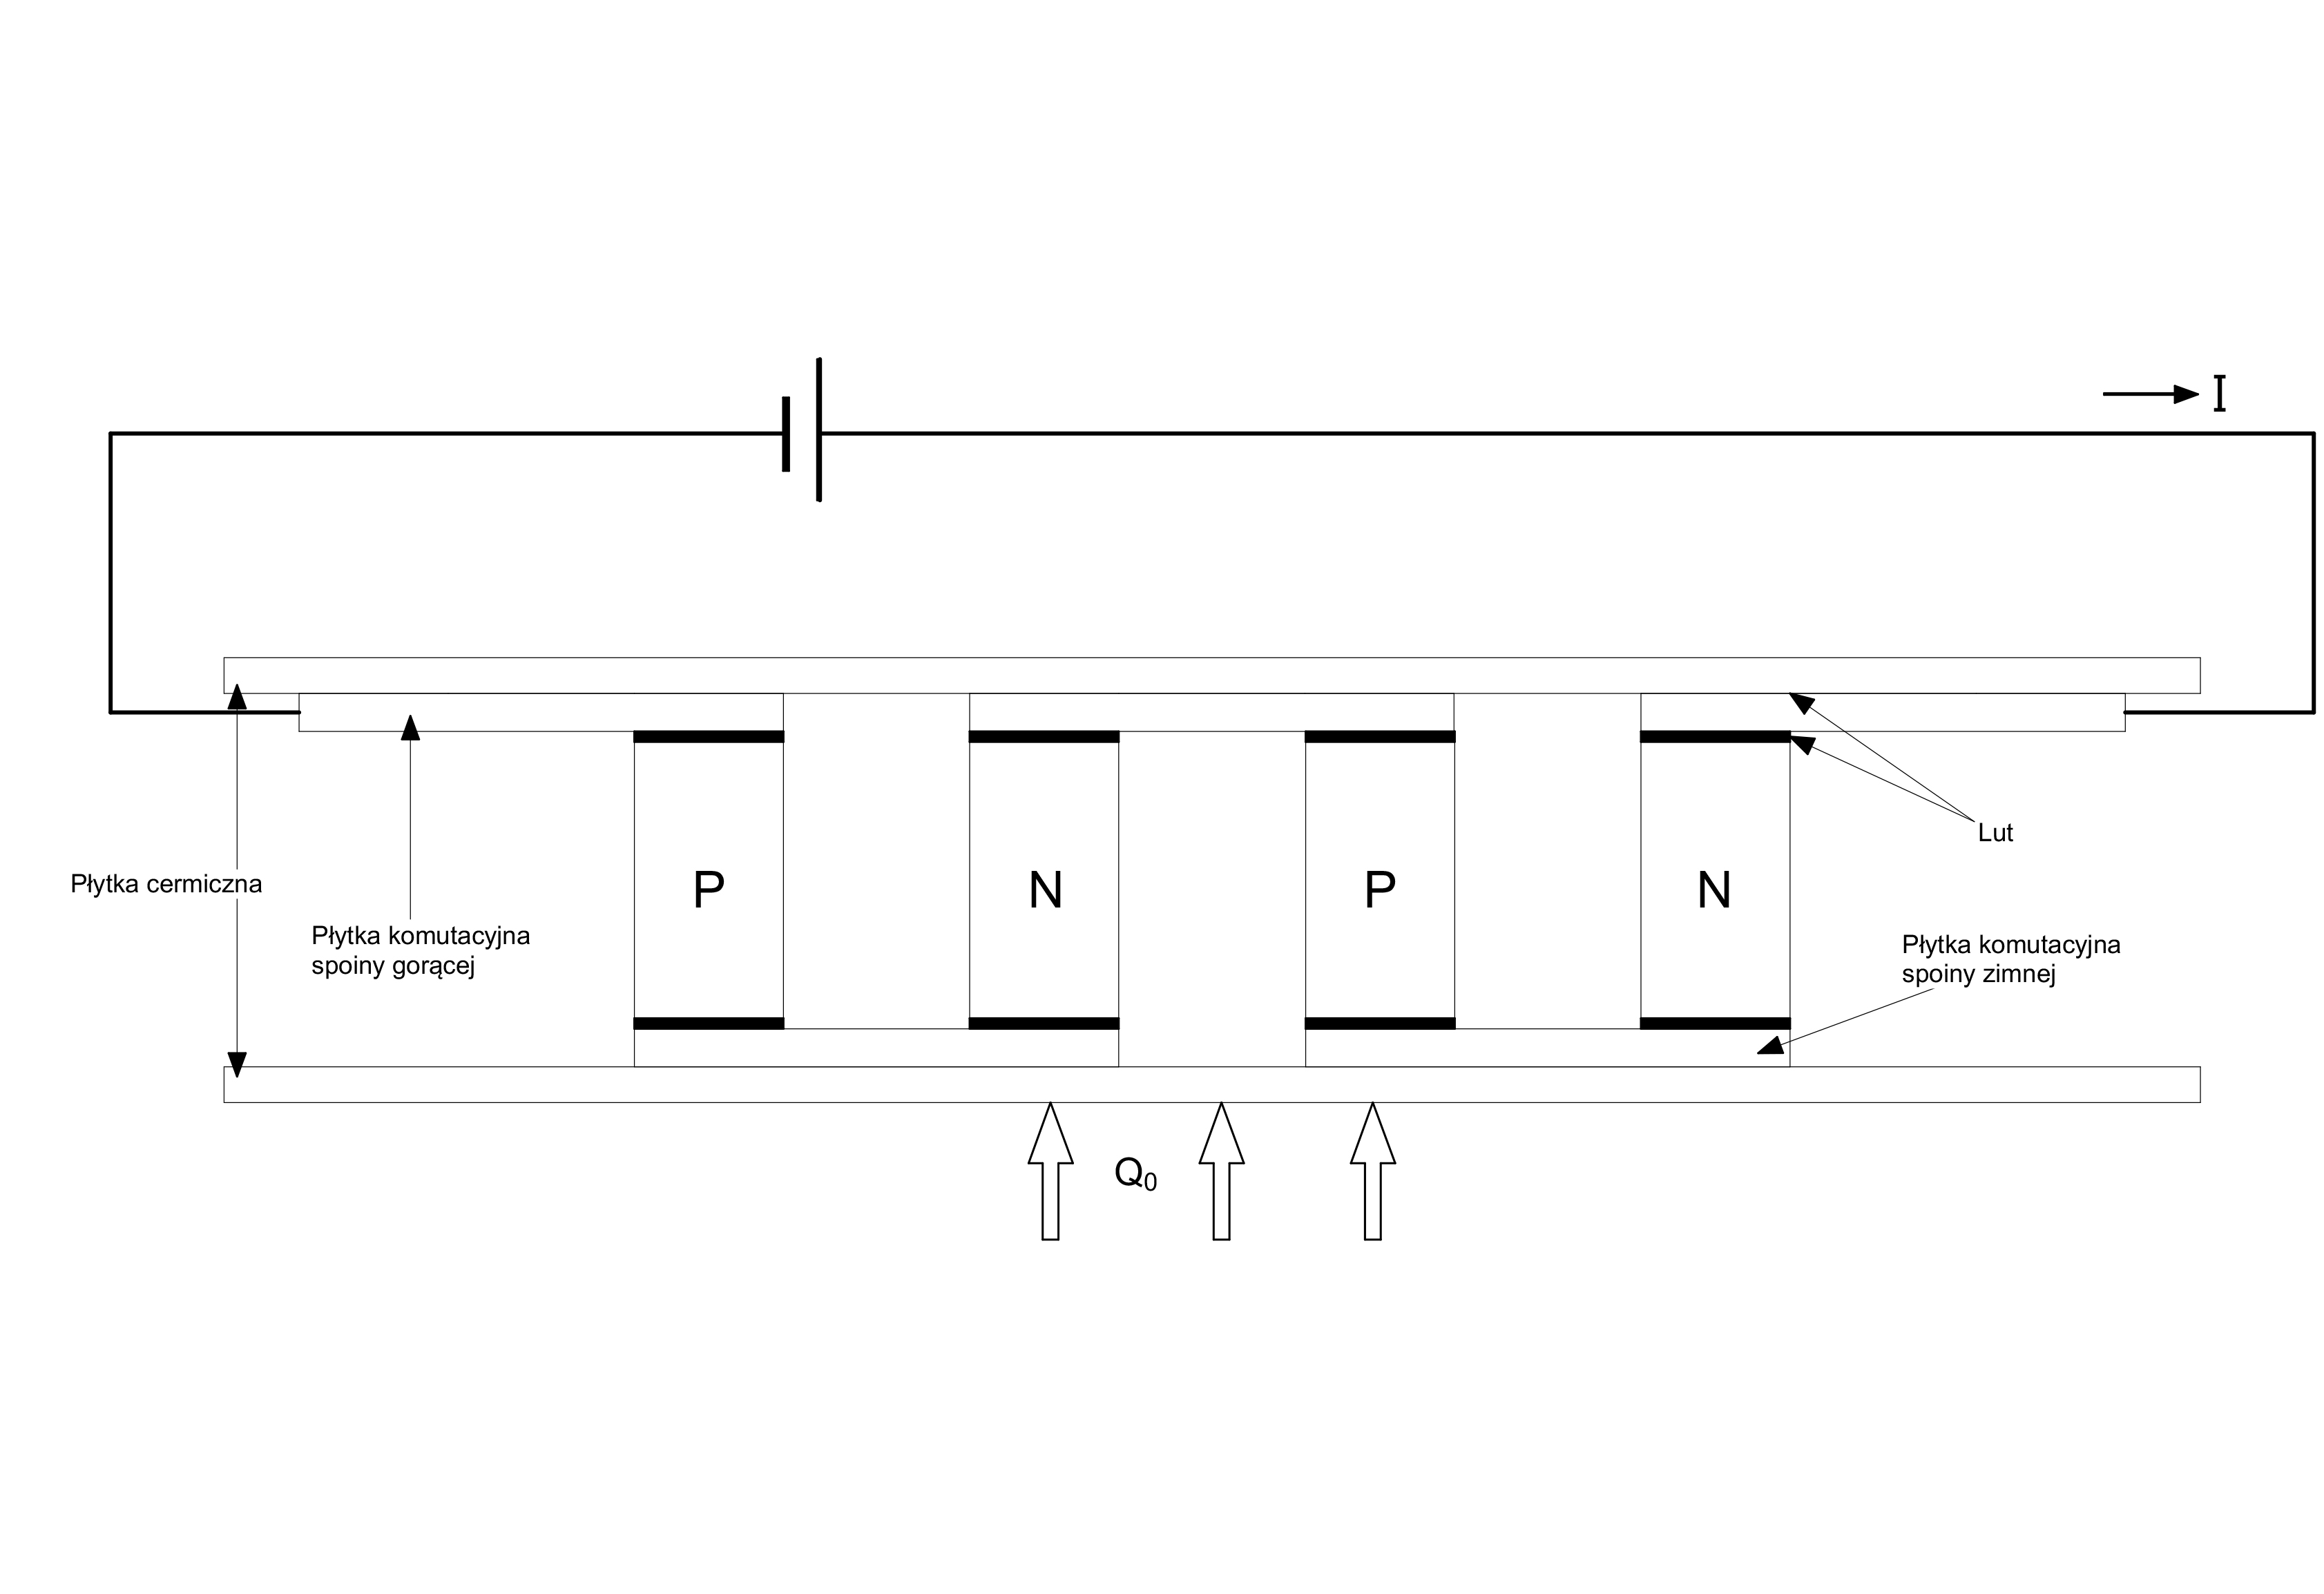
\includegraphics[width=\textwidth]{modul_peltiera.jpg}
    \caption{Schemat ideowy modułu Peltiera}
\end{figure}

Półprzewodnik typu „p” nie ma w swojej strukturze wystarczającej ilości elektronów, aby całkowicie „wypełnić” górny poziom energetyczny, podczas gdy półprzewodnik typu „n” ma ich zbyt wiele. W momencie zasilenia modułu prądem elektrycznym elektrony poruszają się między poziomami energii - co w jednym przypadku wymaga energii (przejście na wyższy poziom energetyczny), a w innym powoduje jej emisję (spadek do niższego poziomu) - w zależności od kierunku przepływu prądu. Zarówno zużyta energia, jak i oddana są w tym przypadku energią cieplną. Na górnej jak i dolnej powierzchni jednocześnie zachodzi pochłanianie ciepła („zimna strona”) i jego oddawanie („gorąca strona”). Dlatego działanie modułów termoelektrycznych często jest porównywane do działania pompy cieplnej.

Ilość ciepła, które można transportować w ten sposób, zależy od natężenia przyłożonego do termoelementu prądu elektrycznego. Można zaobserwować fakt, że gdy prąd przepływa przez system, pewna ilość ciepła powstaje również w samym module (z powodu rezystancji elektrycznej powstaje ciepło Joule'a). Z tego powodu każdy moduł Peltiera charakteryzuje się  pewną maksymalną wydajnością cieplną.

Ważną cechą jest również możliwość łączenia modułów tak, aby „zimna” strona następnego modułu przylegała do „gorącej” strony poprzedniego modułu,
co skutkuje uzyskaniem wyższej wydajności. Biorąc pod uwagę ciepło wytwarzane przez rezystancję prądu elektrycznego, który jest również odprowadzany do „gorącej” strony, takie połączenia są zwykle wykonywane w sposób piramidalny - tak że końcowa powierzchnia emitująca ciepło jest większa niż powierzchnia pochłaniająca. Takie połączenie modułów termoelektrycznych, pod względem zwiększenia wydajności stanowi alternatywę dla zwiększenia prądu przepływającego przez system.

Z uwagi na dużą ilość energii cieplnej(od kilkunastu do nawet kilkuset wat) oddawanej przez "gorącą" stronę, zaleca się stosowanie dodatkowego chłodzenia do ogniw. Najczęściej wykorzystuje się w tym celu radiatory które mogą być dodatkowo wentylowane. Ważne jest również użycie pomiędzy ogniwem a elementem odprowadzającym ciepło pasty przewodzącej która poprawia przepływ ciepła. Wykorzystanie dodatkowych form odprowadzania ciepła ma szczególne znaczenie w przypadku łączenia termoelementów kiedy energia cieplna emitowana przez nie kumuluje się na każdym kolejnym poziomie. 

\subsection{Parametry modułów termoelektrycznych}

W większości literaury parametry ogniw termoelektrycznych są dzielone na dwie grupy: użytkowe i konstrukcyjne. Jednym z głównych parametrów ogniw jest ich maksymalna wydajność chłodnicza $Q_{0(\max)} [W]$ i wytwarzana maksymalna różnica temperatur pomiędzy zimną a ciepłą stroną ogniwa $\Delta T_{\max} [^{\circ} C]$

$Q_{0(\max)}$ wyznaczane jest przy stałej temperaturze górnego źródła ciepłą(z zasady $T_{gor}=+27^\circ C$)[1] i przy zerowej różnicy temperatur pomiędzy stroną zimną a ciepłą modułu czyli $\Delta T_{\max} = T_{gor} - T_z = 0 [^{\circ} C]$. $\Delta T_{\max}$ wyznaczane jest gdy ogniwo nie jest cieplnie obciążone, wtedy gdy wartość $Q_0 = 0$ i gdy temperatura strony gorącej jest stała.

Przedstawione dwie podstawowe wartości odpowiadają punktom przecięcia $Q_0 (\Delta T)$ z osiami układów współrzędnych[1]. Ważną wielkością umieszczaną w charakterystyce każdego modułu jest również $I_{opt}$ jak i inne ważne parametry eksploatacyjne takie jak np. napięcie zasilania czy opór elektryczny modułu.

Oporem prądu zmiennego jest nazywana rezystancja występująca przy $\Delta T = 0$ a więc przy zerowej różnicy temperatur pomiędzy stroną gorącą a zimną ogniwa. Przyjęło się ,że opór taki przyjmuje oznaczenie $R_\sim$, opór prądu stałego jest oznaczany natomiast symbolem $R_=$. Z powodu działania elektrodynamicznej siły Seebecka opór elektryczny termoelementu znacząco zmniejsza się wraz z wzrostem temperatury spoin. Dlatego rozróżniane są różne rezystancje. Opisane wartości opisuje zależność:
\begin{equation}
    U = IR_ = (\text{przy założeniu } \Delta T = \text{const})
\end{equation}

Z kolei paramertry kostrukcyjne modułów termoelektrycznych to między innymi:
\begin{itemize}
    \item wymiary modułu (wysokość, szerokość i długość podawana w milimetrach),
    \item masa modułu (podawana w gramach),
    \item materiał z którego ogniwo zostało wykonane,
    \item ilość naprzemiennie ułożonych złącz p-n,
    \item przewidywany czas pracy lub średni okres lat działania,
    \item maksymalna ilość przełączeń trybów pracy (grzanie/chłodzenie).
\end{itemize}

\subsubsection{Parametr Z modułu i jego pomiar}
Z przytoczonych wyżej informacji wynika, że materiał z którego wykonane są złącza p-n powinien mieć jak anajmniejszą rezystancję i przewodność cieplną a jak najlepsze właściwości związane z zjawiskiem Peltiera. Niestety obe te wymagania wzajemnie się wykluczają.

W celu uzyskania jak najmniejszego oporu modułu termoelektrycznego jego złącza powinny mieć jak największy przekrój i być jak najniższe, jednakże takie rozwiązanie spowoduje szybkie nagrzewanie się strony zimnej od strony gorącej. Dlatego konstrukcja modułu termoelektrycznego wymaga znalezienia złotego środka pomiędzy opornością a wysokością złącz.

W celu wyznaczenia dobroci materiału i jego przydatności do budowy ogniw Peltiera wprowadzono parametr $Z$ którego pomiaru dokonuje się metodą Harmana:
\begin{equation}
    Z = \frac{\alpha^2}{kR}
\end{equation}
gdzie: \\
$k$ - współczynnik przenikania ciepła, \\
$R$ - wartość oporu elektrycznego, \\
$\alpha$ - średnia wartość współczynnika siły termoelektromotorycznej dwóch gałęzi w przedziale temperatur $T_{gor}-T_z$. \\

Z dotychczasowo znanej literatury wynika[1], że najlepszą dobrocią charakteryzuje się wyżej wspomniany półprzewodnik tellurek bizmutu - $Bi_2 Te_3$.

\subsubsection{Pomiar i wyznaczenie maksymalnej różnicy temperatur $\Delta T_{\max}$}

Pomiaru maksymalnej różnicy temperatur strony zimnej i gorącej modułu termoelektrycznego dokonuje się za pomocą systemu składającego się z bardzo dobrze chłodzonej podstawy. Chłodzenie najczęściej jest realizowane przy pomocy radiatora dodatkowo chłodzonego wodą bądź powietrzem której temperatura jest utrzymywana na stałym poziomie. Do połączenia modułu z radiatorem stosuje się pastę termoprzewodzącej która poprawia przewodnictwo cieplne układu. Bezpośrednio przy stronie zimnej jak i gorącej modułu w odpowiednich zagłębieniach znajdują się termparary które mierzą $T_{gor}$ oraz $T_{ch}$ modułu. W przestrzeni w której znajduje się badany obiekt w celu zmniejszenia obciążenia cieplnego stosuje się obniżenie ciśnienia do $10^{-3} \dots 10^{-4}$ mmHg. Dalsze obniżanie ciśnienia nie ma wpływu na polepszenie dokładności wyników pomiarów. W celu dalszej poprawy wyników stosuje się ograniczenie dostępności światłdo obiektu bądź otoczneie całego systemu odpowiednim ekranem chłodzącym którego temperatura będzie utrzymywany blisko $T_{ch}$. Poprzez stopniowe zwiększanie natężenia prądu wyznaczyć można wyznaczyć minimalną temperaturę strony zimnej. Pozwala to na wyznaczenie $\Delta T_{\max}$ i parametru $Z$. Wykorzystanie tej metody do wyznaczenia parametru $Z$ nie uwzględnia ciepła Thomsona[1], co powoduje zawyżenie wartości $Z$.

Na podstawie[1] w celu dokładnego wyznaczenia parametru $Z$ należy skorzystać z poprawionego wzoru:
\begin{equation}
    Z = 2 \Delta T_{\max}/{T_{ch}^2}_{(\min)}[1/3(\Delta T_{\max}/T_{ch}(\beta/\alpha))]
\end{equation}
gdzie:\\
$\beta$ - współczynnik Thomsona z równania (2.7). \\

A więc aby precyzyjniej wyznaczyć parametr $Z$ należy znać $\alpha$ orza $\beta$. Aby uzyskać jak najbardziej dokładne wyniki należy zadbać aby chłodzenie badanego modułu było jak najlepsze poprzez chłodzenie powietrzem bądź wodą. Zabieg taki pozwoli na ograniczenie podgrzewania strony grzejącej ogniwa przez stronę chłodzącą.

Zmierzone $\Delta T_{\max}$ przedstawioną powyżej metodą(pomiar dokonywany w próżni) z reguły przedstawiane jest charakterystykach modułów termoelektrycznych. Te same badania wykonane bez wykorzystania próżni pozwala na uzyskanie wyników około 20\% mniejszych.

\subsubsection{Wyznaczenie i pomiar $Q_{0(\max)}$ modułu}

Stanowisko do pomiaru parametru $Q_{0(\max)}$ modułu termoelektrycznego wygląda podobnie do stanowiska do pomiaru $\Delta T_{\max}$ z tą różniczą ,że zamiast stosowania próżni stosuje się odpowiednią izolację termiczną. Zabieg ten wykonuje się w celu ograniczenia wpływu ciepła pochodzącego z otoczenia na badany moduł. Najczęściej wykorzystywanym materiałem do izolacji obiektu jest poliuretan o grubości do 50 mm. Moduł termoelektryczny zasilany jest przy pomocy zasilacza, pozwalającego w precyzyjny sposób kontrolować napięcie i natężenie prądu elektrycznego. Wymnożenie napięcia i natężenia prądu pozwala otrzymać moc elektryczną. Przyjmuje się ,że 100\% tej mocy zamienia się na ciepło ,które przejmuje moduł[1]. Zastosowane termoelektryczne czujniki temperatury bezpośrednio przy stronie chłodnej i gorącej modułu pozwalają na bieżący pomiar temperatury. Poprzez równomierne zwiększanie napięcia, należy ustalić stan równowagi w którym $\Delta T = 0$ a więc temperatura strony gorącej modułu zrówna się z temperaturą strony chłodnej. Uzyskana w taki sposób moc jest maksymalną wydajnością chłodniczą modułu termoelektrycznego $Q_{0(\max)}$. Ważne jest aby wszystkie parametry wyznaczać przy wspólnych warunkach początkowych modułu.

\subsection{Wykorzystanie ogniw Peltiera}

Ogniwa Peltiera dzięki swojej nieskomplikowanej budowie, małym rozmiarom oraz niezawodności znalazły szerokie zastosowanie jako pompy cieplne. Ogniwa stosuje się do budowy urządzeń chłodniczych wykorzystywanych w sprzętach gospodarstwa domowego jak i w zaawansowanych technologicznie systemach chłodzenia wykorzystywanych w przemyśle oraz medycynie. Stanowią one doskonałe uzupełnienie sprzętu chłodniczego gdy zależy nam na pracy układu w różnych położeniach jak i braku szkodliwych substancji (np. freonu).

Najczęściej moduły Peltiera stosuje się:
\begin{itemize}
    \item chłodzenie nagrzewających się urządzeń elektrycznych
    \item komory klimatyczne
    \item chłodzenie diod wykorzystywanych w laserach wysokich mocy
    \item przenośne i stacjonarne urządzenia klimatyzacyjne
    \item termostaty wykorzystywane w akwarystyce
    \item przenoścne lodówki
\end{itemize}

Niezwykle ważnym zastosowaniem ogniw Peltiera jest również zastosowanie ich do produkcji prądu elektrycznego korzystając z zjawiska Seebecka. Ciekawostką jest fakt, że niektóre bezzałogowe statki kosmiczne (w tym łazik Curiosity Mars) wykorzystują radioizotopowe generatory termoelektryczne (RTG), które przekształcają energię cieplną w energię elektryczną za pomocą efektu Seebecka. Urządzenia mogą przetrwać kilka dziesięcioleci, ponieważ są napędzane przez rozpad wysokoenergetycznych materiałów radioaktywnych.

\chapter{Oprogramowanie}
\section{LOGO! SoftComfort}
Pakiet LOGO! SoftComfort pozwala na wygodne programowanie w jednym środowisku programistycznym sterowników serii: LOGO! oraz współpracujących z nimi paneli operatorskich i innych urządzeń producenta. Pakiet oprogramowania zawiera wiele udogodnień i rozwiązań ułatwiających pracę z sterownikami. Miedzy innymi posiada przejrzysty interfejs graficzny pozwalający na pracę bez konieczności posługiwania się samym urządzeniem LOGO!. W pracy w celu stworzenia programu posłużono się schematem drabinkowym(Ladder Diagram) jednakże program pozwala również na programowanie przy pomocy bloków funkcjonalnych.

Dodatkowym udogodnieniem jest możliwość symulacji działania całego układu w komputerze PC. Program również można testować online co daje możliwość podejrzenia zmian stanów wejść i wyjść cyfrowych oraz zmiennych procesowych w trybie sterownika "RUN". Przenoszenie napisanego programu z komputera PC do sterownika PLC i odwrotnie odbywa się przy pomocy przewodu Ethernet.

\section{Baza danych pomiarowych}
Wykorzystanie pakietu Microsoft Office a konkretnie programu Excel pozwala na utworzenie prostej bazy danych. Program Excel do poprawnej pracy z sterownikiem PLC wymaga pobrania narzędzia LOGO!AccessTool dostępnego na stronie Siemensa. Następnie należy zaimportować dodatek LOGO!AccessTool do programu Excel i go skonfigurować miedzy innymi określić w jakich odstępach czasowych dane mają być pobierane z sterownika.  Poprawna instalacja i konfiguracja narzędzia pozwala na odczyt i zapis danych z czujników pomiarowych w czasie rzeczywistym. 

Dzięki pakietowi office jest możliwa również dalsza interpretacja zebranych pomiarów. Program Excel daje możliwość utworzenia tabel czy wykresów. Analiza i badanie zebranych danych pomiarowych z obiektu jest przedstawiona w dalszej części pracy.

\chapter{Realizacja stacji badawczej z komorą termiczną}
\section{Opis obiektu}

W celu zrealizowania układu pozwalającego na badanie i regulacje temperatury z wykorzystaniem ogniw Peltiera został zbudowany obiekt badawczy. Urządzenie składa się z stelażu wykonanego z profili aluminiowych na którym zostały osadzone urządzenia sterujące, pomiarowe oraz wykonawcze. Dodatkowo została wykonana zamknięta komora badawcza z szkła akrylowego o grubości 6$mm$. która ogranicza emisję ciepła do otoczenia. Istnieje możliwość wyjęcia całego systemu chłodzącego w skład którego wchodzi ogniwo wraz z radiatorami i wentylatorami. Aby tego dokonać należy odłączyć złącze, odkręcić śrubki motylkowe i delikatnie wysunąć górną część komory wraz z wszystkimi elementami wykonawczymi. Zabieg ten może zostać wykonany w wypadku konieczności konserwacji urządzenia, wyczyszczenia komory chłodzącej bądż też wymiany ogniwa Peltiera. 

Temperatura wewnątrz komory badawczej może być zakłócana poprzez zastosowanie czterech sterowanych analogowo rezystorów wysokich mocy. Każdy z rezystorów charakteryzuje się mocą 50W. Urządzenie pozwala na regulację mocą grzewczą rezystorów w zakresie 0-100\%. Zasilanie wszystkich urządzeń realizowane jest przy pomocy zasilacza 24 V.

Elementami pomiarowymi które są odpowiedzialne za mierzenie temperatury  w czasie rzeczywistym są trzy czujniki temperatury ($T_1, T_2, T_3$) które zostały zainstalowane bezpośrednio przy stronie gorącej oraz zimnej modułu jak i wewnątrz komory termicznej. Takie rozwiązanie pozwala na zmierzenie różnicy temperatur po stronie gorącej i chłodnej ogniwa oraz wewnątrz zbudowanej komory termicznej. Dodatkowo w celu odprowadzania z ogniwa ciepła oraz zimna w układzie zastosowane zostały radiatory które wspomagane są przez wentylatory obrotowe. Takie rozwiązanie pozwala na efektyne chłodzenie ogniwa w trakcie pracy z maksymalnym obciążeniem cieplnym.

W celu sterowania temperaturą wewnątrz komory termicznej został zastosowany sterownik cykliczny PLC serii LOGO!8 wraz z modułem analogowym. Zastosowanie sterownika pozwala na nieprzerwaną i bezawaryjną pracę układu wraz z możliwością precyzyjnego utrzymywania zadanych parametrów. Dodatkowo dzięki wspieraniu przez sterownik pakietu Microsoft Office możliwe jest łatwe zapisywanie mierzonych parametrów w bazie danych i ich późniejsza analiza.Całym obiektem można sterować na dwa sposoby: ręcznie z wykorzystaniem zadajnika prądowego wraz z panelem HMI LOGO! TDE lub automatycznie wykorzystując sterownik. Możliwe jest podłączenie do układu komputera PC przy pomocy kabla Ethernet. 

Wszystkie przewody sygnałowe oraz sterujące zastosowane w obiekcie zostały poprowadzone w zębatych listwach prowadzących. Wszystkie elementy sterujące jak i zasilające zostały osadzone na listwach przemysłowych. Panel operatorki oraz panel sterujący zadajnika prądowego został osadzony w pleksi. Zastosowanie takich rozwiązań pozwoliło zachować należytą estetykę układu i poprawić jego przejżystość(rys. 3.1).

\begin{figure}
    \centering
    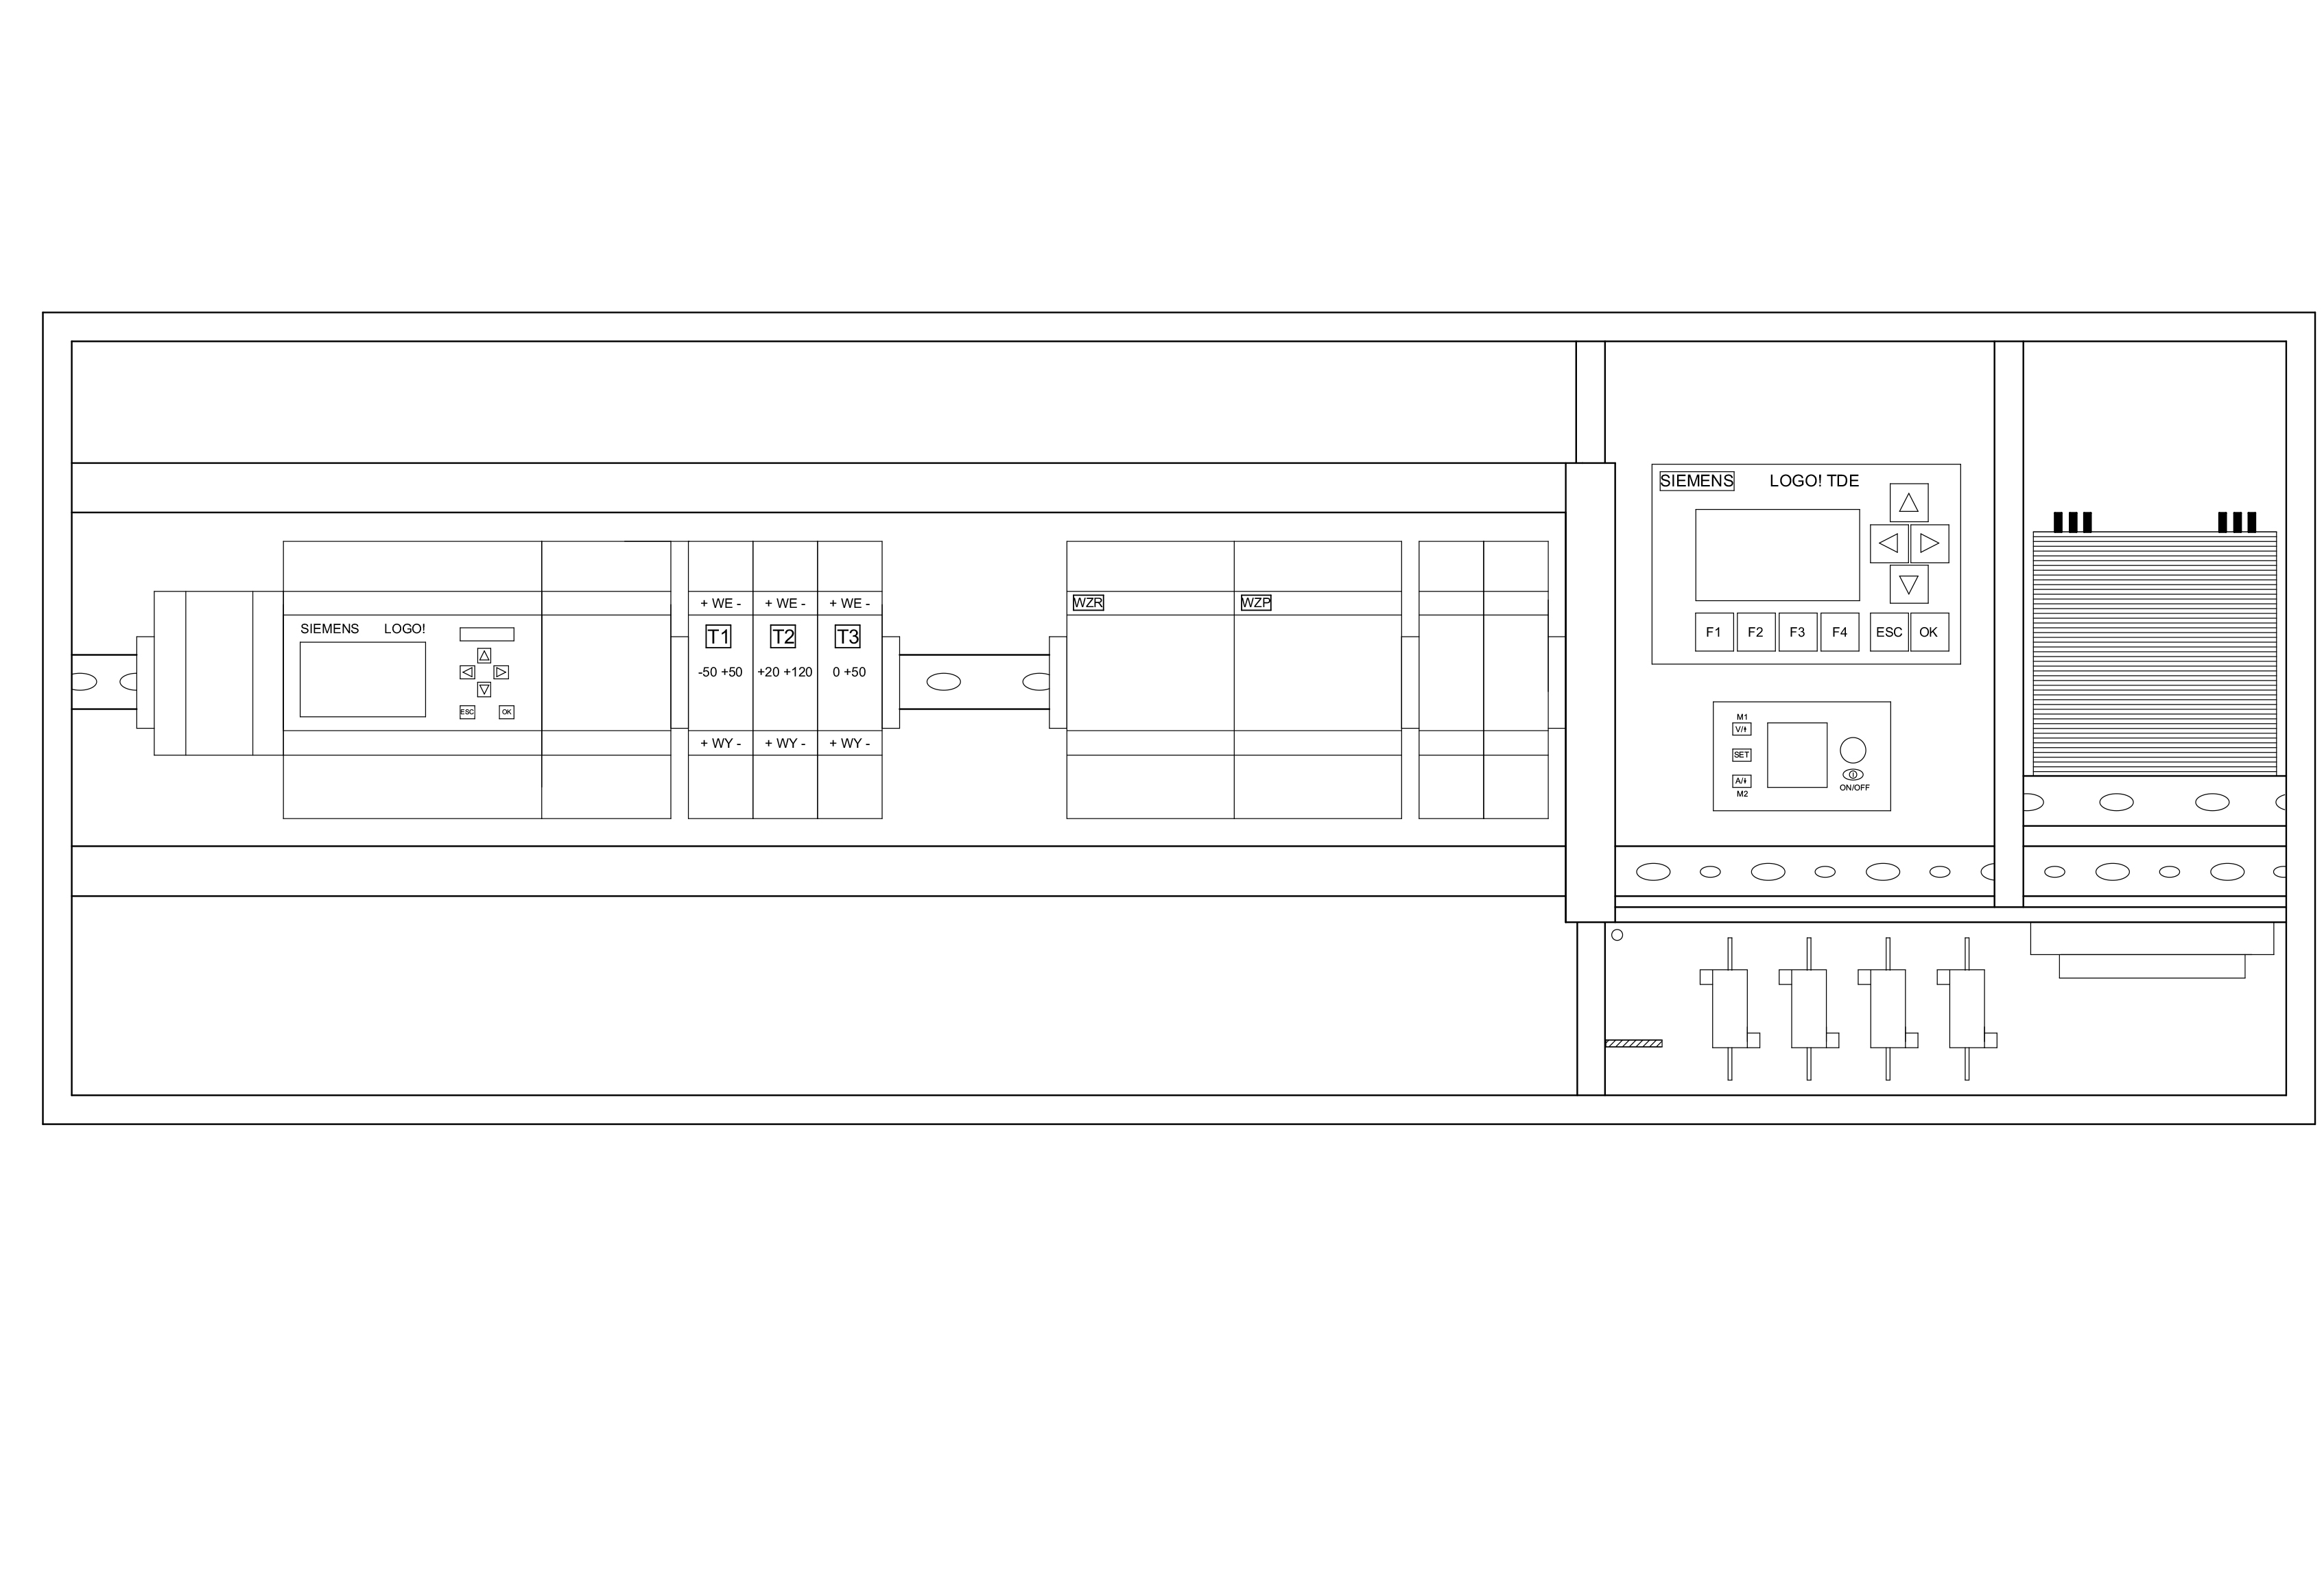
\includegraphics[width=\textwidth]{obiekt_front.jpg}
    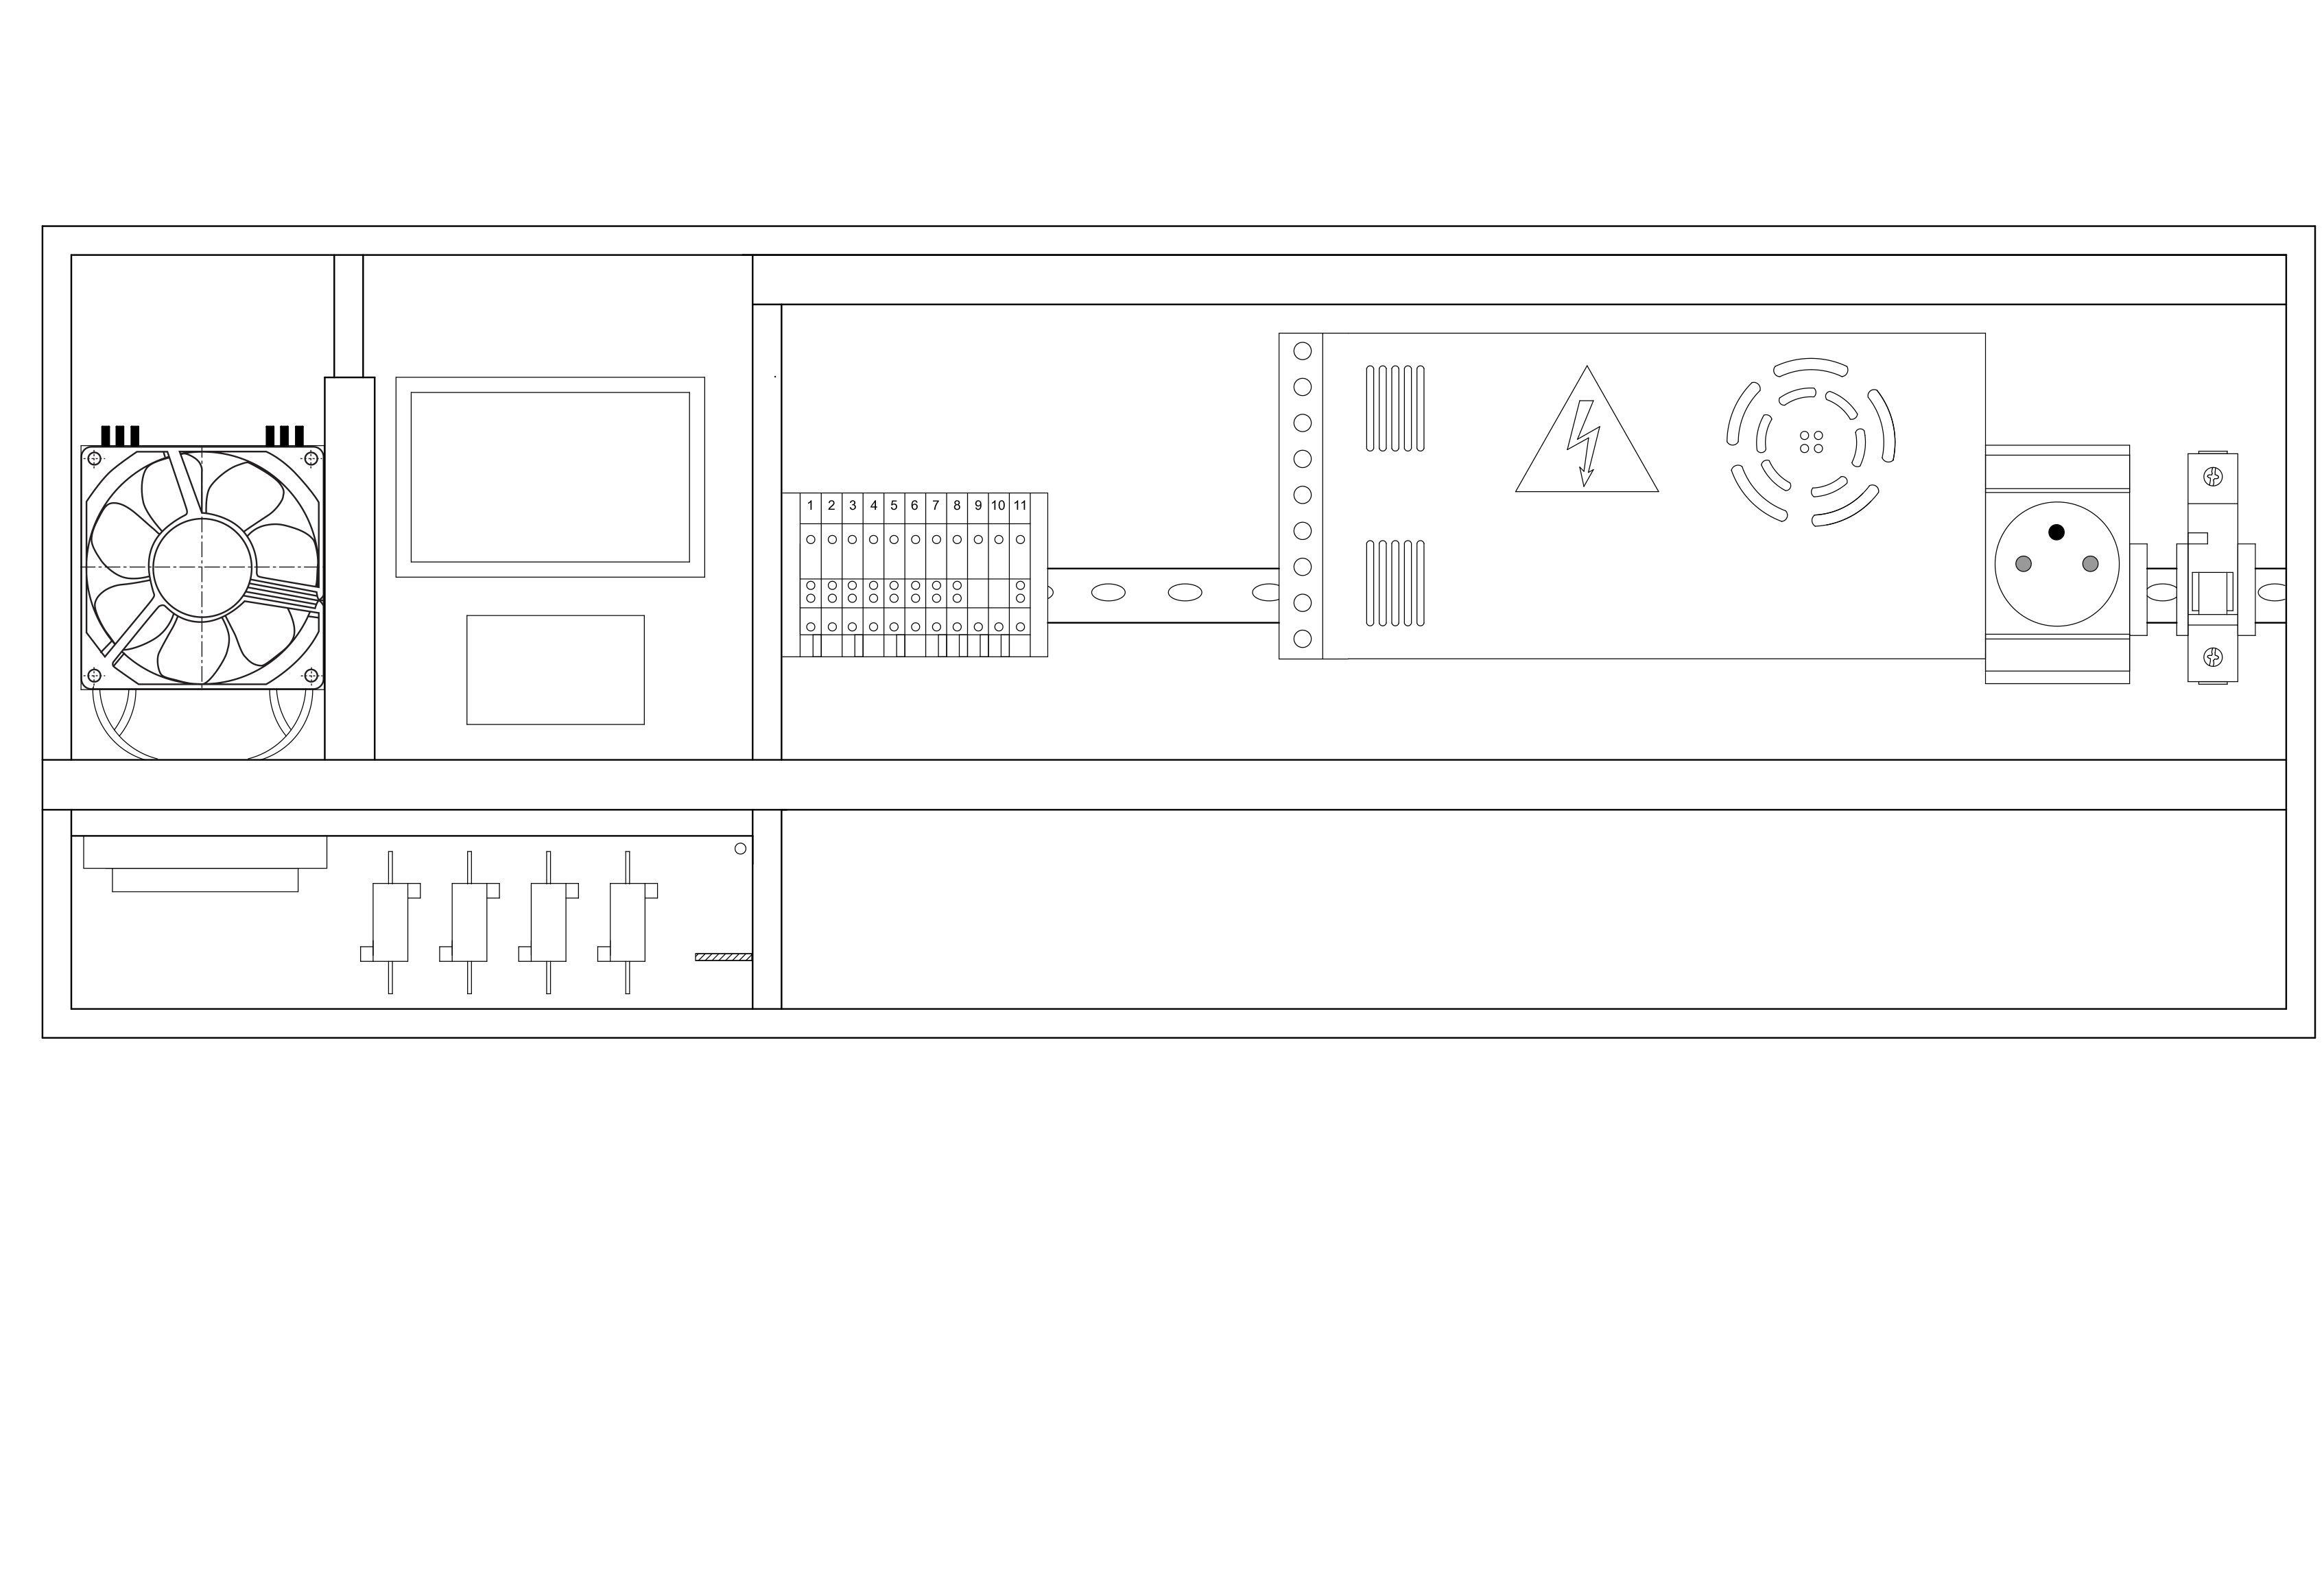
\includegraphics[width=\textwidth]{obiekt_back.jpg}
    \caption{Schemat ideowy urządzenia}
\end{figure}

\section{Wykaz elementów}
Poniżej zostały przedstawione kolejno urządzenia odpowiedzialne za sterowanie układem, urządzenia wykonawcze oraz urządzenia pomiarowe. Przedstawione również zostały sygnały które każde z urządzeń odbiera i generuje wraz z krótkim ich opisem.
\subsection{Urządzenia sterujące}
Do urządzeń sterujących układem zaliczany jest sterownik PLC: LOGO!8 wraz z modułem analogowym oraz przetwornica napięcia typu: DPS5015 pozwalająca manualnie ustawić napięcie i natężenie prądu płynącego przez badane ogniwo termoelektryczne. Dodatkowo w układzie zastosowany został panel operatorski LOGO! TDE pozwalający na odczytywanie bieżących pomiarów temperatury. Panel umożliwia również sterowanie układem w trybie ręcznym.

\subsubsection{LOGO! 0BA8 (LOGO! 12/24RCE)}
LOGO! jest uniwersalnym modułem logicznym firmy Siemens który pozwala na zintegrowanie sterowania wraz z zasilaniem oraz interfejsem modułów rozszerzeń. Również istnieje możliwość podłączenia opcjonalnego modułu wyświetlania tekstu(TDE).

\begin{figure}
    \centering
    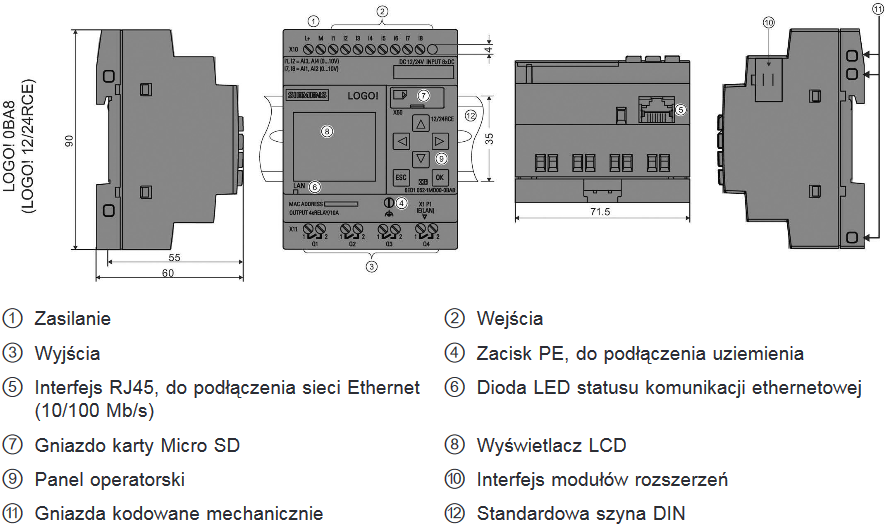
\includegraphics[width=\textwidth]{Sterownik_LOGO!.PNG}
    \caption{Sterownik LOGO! 0BA8 (LOGO! 12/24RCE)[3]}
\end{figure}

\subsubsection{LOGO! AM2 AQ (0/4\dots20 mA or 0 \dots 10 VDC)}
LOGO! AM2 AQ jest modułem analogowym zasilanym przez 24V DC. Posiada dwa wyjścia analogowe 4-20ma lub 0-10 VDC. W pracy moduł został wykorzystany do regulacji mocy rezystorów wewnątrz komory termicznej oraz regulacji prądu przepływającego przez ogniwo Peltira.

\begin{figure}
    \centering
    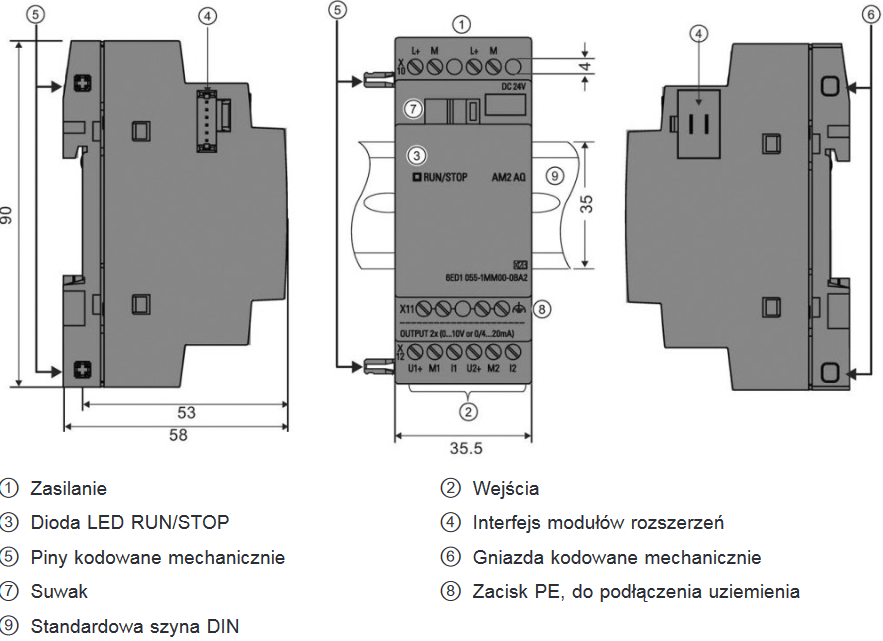
\includegraphics[width=\textwidth]{Modul_analogowy.PNG}
    \caption{Moduł analogowy LOGO! AM2 AQ (0/4\dots20 mA or 0 \dots 10 VDC)[3]}
\end{figure}

\subsubsection{Panel operatorski LOGO! TDE}

Użycie zintegrowanego z sterownikiem panelu operatorskiego LOGO! TDE pozwala na intuicyjne sterowanie całym układem. Sterowanie odbywa się przy pomocy czterech pulpitów operatorskich wykonanych w programie LOGO! SoftComfort. Panel operatorski składa się z czterech przycisków funkcyjnych, przycisku "ESC" oraz "ENTER" oraz czterech strzałek kierunkowych.

\begin{figure}
    \centering
    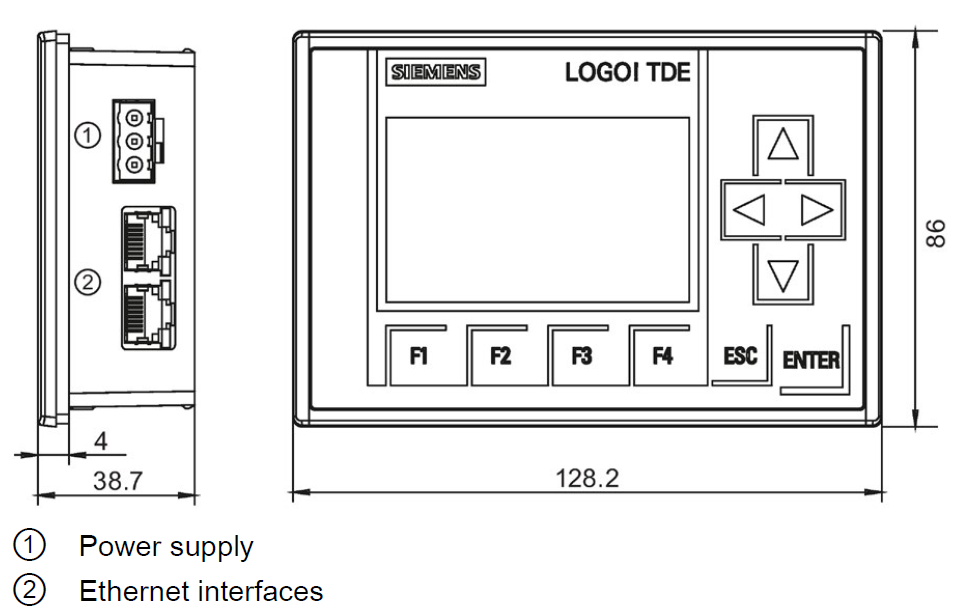
\includegraphics[width=\textwidth]{HMI.PNG}
    \caption{Panel operatorski LOGO! TDE [3]}
\end{figure}


\subsubsection{Przetwornica napięcia 0-50V 750W DPS5015}

Zasilacz DPS5015 oferuje bardzo wysoką precyzję i dokładność. Regulowane wyjście osiąga do 50V natężenia lub 15A napięcia i może być skonfigurowane w precyzyjnych krokach co 10mV lub 1mA. Zasilacz dodatkowo jest wyposażony w pamięć parametrów awaryjnego wyłączenia oraz programowalną pamięć danych. Urządzenie charakteryzuje się prostą obsługą, kolorowy wyświetlacz dostarcza prostych informacji między innymi mogą to być aktualne wartości napięcia i natężenia prądu wraz z mocą wyjściową[4].

\begin{figure}
    \centering
    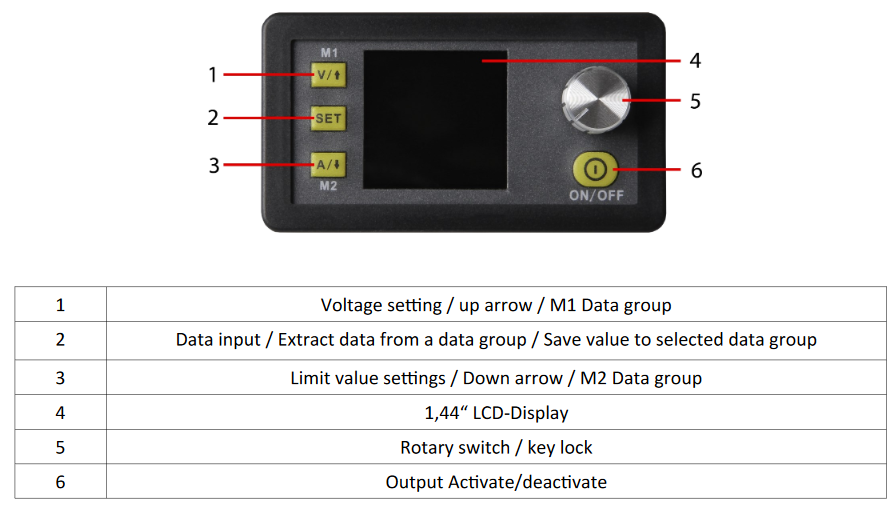
\includegraphics[width=\textwidth]{Przetwornica_napiecia.PNG}
    \caption{Przetwornica napięcia 0-50V 750W DPS5015[4]}
\end{figure}

\subsubsection{Analogowy wzmacniacz mocy}
Wzmacniacze wykorzystane w układzie służą do regulacji natężenia prądu płynącego przez moduł termoelektryczny oraz rezystory. Wykorzystany w obiekcie model wzmacniaczy to M12N3 pozwalają one na uzyskanie maksymalnego prądu pracy ciągłej 20A co w zupełności wystarcza do zasilenia zarówno rezystorów jak i ogniwa Peltiera. Pozwalają one na regulację mocy wyjściowej w zakresie 0-99\%. Wzmacniacz rezystorów jest zasilany bezpośrednio z zasilacza impulsowego prądu stałego. Wzmacniacz ogniwa Peltiera jest zasilany z przetwornicy napięcia. Wykorzystanie regulatorów zapewnia płynną regulację mocy wyjściowej charakteryzują się niezawodnością oraz małymi gabarytami. 

\subsection{Urządzenia wykonawcze}

Do grupy urządzeń wykonawczych wykorzystanych w projekcie które wpływają na temperaturę w komorze termicznej możemy zaliczyć: ogniwo Peltiera, przekaźniki, rezystory oraz radiatory wspomagane przez wentylatory. Dodatkowo w tej części zostały opisane elementy zasilające układ wraz z zastosowanymi urządzeniami bezpieczeństwa.
\subsubsection{Ogniwo Peltiera}
W układzie zastosowane zostało ogniwo Peltiera typu TEC1-12715. Nominalna wartość napięcia zasilania wybranego ogniwa wynosi 12 V(dopuszcza się napięcie do 15,5 V). Maksymalny pobór prądu wynosi natomiast 11.8 A co pozwala na pracę ogniwa z maksymalną odprowadzaną mocą do 142W. Ogniwo charakteryzuje się opornością od 0,8\ohm do 0,9\ohm.
\subsubsection{Przekaźniki}
W pracy zostały użyte dwa przekaźniki RMP84 osadzone w gniazdach typu GZMB80. Pierwszy z nich został wykorzystany do przełączania kierunku przepływu prądu przez ogniwo Peltiera a tym samym zmianę polaryzacji na nim. Pozwala to na zmiany pracy ogniwa(grzanie, chłodzenie). Drugi przekaźnik pozwala na zmianę trybów pracy układu z ręcznego na automatyczny. Przekaźnik zapobiega również włączeniu dwóch trybów pracy jednocześnie i poboru prądu przez ogniwo jednocześnie z sterownika i zadajnika prądowego. Wybrano gniazda przekaźnikowe wyposażone w diody które zapobiegają "cofaniu" się prądu z układu na sterownik w momencie gdy np. układ zostanie wyłączony a temperatury strony zimnej i ciepłej ogniwa będą znacznie się różnić. W takim wypadku diody powodują rozproszenie się prądu.
\subsubsection{Wentylatory}
W układzie zastosowane zostały dwa wentylatory firmy Saunon. Większy do wspomagania odprowadzania ciepła z radiatora strony ciepłej układu oraz mniejszy do strony zimnej układu. Oba wentylatory zasilane są przy pomocy dwóch przewodów napięciem 24V i generują 34 dBA hałasu. Większy wentylator pracuje z prędkością obrotową wynoszącą 2200 RPM co pozwala na przetłaczanie 127.3 $m^3/h$ powietrza. Mniejszy natomiast wspomagający odprowadzenie zimnego powietrza z ogniwa oraz rozprowadzenie go po komorze termicznej pracuje z prędkością obrotową wynoszącą 3000 RPM i wydajnością wynoszącą 87.4 $m^3/h$.
\subsubsection{Radiatory}
Do odprowadzenia ciepła ze strony grzejącej ogniwa oraz zimna ze strony chłodnej wykorzystano dwa żeberkowe radiatory wykonane z aluminium. Do odprowadzania ciepła ze strony gorącej ogniwa wykorzystano radiator SilentiumPC Fera 3. Radiator został wykonany z wykorzystaniem technologi HE (High Efficiency) wyposażony jest w cztery rurki cieplne które dotykają bezpośrednio modułu i tym samym poprawiają odprowadzanie ciepła zapewniając niższe temperatury. Wykorzystany radiator pozwala na odprowadzenie 180W mocy cieplnej co w zupełności wystarcza dla zastosowanego ogniwa Peltiera. Do rozprowadzania chłodu wewnątrz komory termicznej użyto prostego radiatora żeberkowanego. 
\subsubsection{Rezystory}
W celu wprowadzenia zakłóceń do układu w komorze termicznej zostały zamontowane cztery przykręcane rezystory drutowe zintegrowane z radiatorami. Każdy charakteryzuje się mocą 50W i opornością 20\ohm. Wszystkie rezystory zostały połączone równolegle i w pracy traktowane są jako jedno źródło ciepła. Regulacji temperatury na rezystorach dokonuje się manualnie przy użyciu panelu operatorskiego TDE lub automatycznie przy pomocy sterownika PLC.
\subsubsection{Zasilanie}
Zasilanie układu zostało zrealizowane przy pomocy stabilizowanego impulsowego zasilacza 24V - 20A - 480W. Wykorzystany zasilacz charakteryzuje się małymi gabarytami w porównaniu do innych transformatorowych zasilaczy oraz  dużą stabilnością napięcia wyjściowego. Dodatkowo na szynie obok zasilacza zostało zamontowane gniazdo elektryczne.
\subsubsection{Bezpieczeństwo}
W układzie został zamontowany główny wyłącznik nadprądowy TDZ 16A charakterystyka B. Koniecznością było zastosowanie wyłącznika 16A z uwagi na natężenie prądu pobierane przez ogniwo i moce jakie generuje. Dodatkowo każdy z rezystorów oraz urządzenia sterujące zostały zabezpieczone przez  bezpieczniki szklane typu F2AL250V. Ogniwo Peltiera dodatkowo zabezpiecza szklany bezpiecznik zwłoczny typu T10AL250V. Wszystkie bezpieczniki szklane zostały zainstalowane w dedykowanych kasetach.

\subsection{Urządzenia pomiarowe}
Urządzeniami mierzącymi w czasie rzeczywistym temperaturę zimnej i ciepłej strony modułu wraz z temperaturą wewnątrz komory termicznej są czujniki temperatur typu: PT0-10. 

PT0-10 składa się z układu cyfrowego przetwornika sygnału na napięcie 0-10V oraz czujnika temperatury DS18B20. Sygnał wyjściowy przetwornika jest proporcjonalny do mierzonej przez czujnik temperatury. Zespół urządzeń PT0-10 pozwala na ograniczenie zakresu mierzonej temperatury do interesujących nas granic pomiarowych. Taki zabieg pozwala zwiększyć rozdzielczość dokonywanych pomiarów w określonym przedziale temperaturowym. Czujnik temperatury T0-92 jest połączony z przetwornikiem przy pomocy trójżyłowego kabla o długości dwóch metrów który można dodatkowo przedłużyć lub skrócić do maksymalnie 0,2m na potrzeby projektu. Jeśli połączenie czujnika z przetwornikiem będzie dłuższe niż 5m powinno być ono dodatkowo ekranowane oraz uziemione w celu minimalizacji zakłóceń pomiarowych na sygnał analogowy. Do wykonywania długich połączeń czujnika z z przetwornikiem producent zaleca stosowanie skrętki z koralikiem ferrytowym. Płytka przetwornika została zamontowana w dedykowanej obudowie typu KMz-105[6].

W zbudowanym urządzeniu zostały wykorzystane trzy układy pomiaru temperatury PT0-10:
\begin{itemize}
    \item T1 - Czujnik umieszczony bezpośrednio pod ogniwem Peltiera pozwalający na pomiar temperatury zimnej strony ogniwa. Zakres mierzonych temperatur wynosi -50\dots50 stopni C.
    \item T2 - Czujnik umieszczony bezpośrednio nad ogniwem Peltiera pozwalający na pomiar temperatury gorącej strony ogniwa. Zakres mierzonych temperatur wynosi 20\dots120 stopni C.
    \item T3 - Czujnik umieszczony wewnątrz komory termicznej. Zakres mierzonych temperatur wynosi 0\dots50 stopni C.
\end{itemize}
Wszystkie układu pomiarowe zasilane są napięciem 24V z sterownika PLC.
\newpage
\begin{table}[h!]
\footnotesize
\begin{tabularx}{\textwidth}{|c|X|X|c|c|}
\hline
\rowcolor{lightgray}
    Lp. & \multicolumn{2}{|c|}{Urządzenie}        & Ilość          & Producent                                    \\\hline
    1.      &LOGO!8 12/24RCE     &Sterownik PLC      &1       &Siemens\\\hline
    2.      &LOGO!8 AM2 AQ-6ED1055-1MM00-0BA2    &Moduł analogowy      &1       &Siemens\\\hline
    3.      &LOGO! TDE    &Panel operatorski      &1       &Siemens\\\hline
    4.      &M12N3    &Wzmacniacz      &2       &CAY Regulatory\\\hline
    5.      &PT0-10    &Czujnik temperatury z przetwornikiem      &3       &Telematic\\\hline
    6.      &DPS5015    &Przetwornica napięcia      &1       &Gotronik\\\hline
    7.      &TEC1-12715    &Ogniwo Peltiera      &1       &Hesta\\\hline
    8.      &24V-20A-480W     &Zasilacz impulsowy     &1       & 	nieokreślony\\\hline
    9.      &RMP84 2012-25-1024-WT      &Przekaźnik     &2       &Relpol\\\hline
    10.      &GZMB80      &Gniazdo przekaźnika     &2       &Relpol\\\hline
    11.      &1F TYP S301 B-16A     &Wyłącznik główny nadprądowy     &1       &Tracon Electric\\\hline
    12.      &F2AL250V      &Bezpiecznik szklany szybki     &5       &Elektropark\\\hline
    13.      &T10AL250V      &Bezpiecznik szklany zwłoczny     &1      &Elektropark\\\hline
    14.      &TS-35 z otwor. 35x7,5x1000mm      &Szyna montażowa     &2      &EBMiA\\\hline
    15.      &PR-0478     &Koryto grzebieniowe 25x25/2000mm     &1      &EBMiA\\\hline
    16.      &PR-0668    &Koryto grzebieniowe 25x40/2000mm     &1      &EBMiA\\\hline
    17.      &3842992888/3000    &Profil, materiał: aluminium, dł. 3000mm, 20 x 20 mm   &1      &Bosch Rexroth\\\hline
    18.      &3842535572   &Klamra, 10mm     &32      &Bosch Rexroth\\\hline
    19.      &3842530285    &Nakrętka do rowków typu T, 10mm     &10      &Bosch Rexroth\\\hline
    20.      &EW 35-383560000    &Wspornik końcowy   &8      &Weidmuller\\\hline
    21.      &1061200000    &Wspornik końcowy   &4      &Weidmuller\\\hline
    22.      &1763940000 WTR 2.5/SI    &Zaciskowa złączka szynowa   &4      &Weidmuller\\\hline
    23.      & WSI 6/LD 10-36V DC/AC -1011300000     &Złączka szynowa bezpiecznikowa   &7      &Weidmuller\\\hline
    24.      &2ESDV-06P; 6 torów     &Łączówka   &2      &Dinkle\\\hline
    25.      &2EHDRD-08P     &Złączka   &2      &Dinkle\\\hline
    26.      &2m$^2$ grubość 6mm    &Plexi bezbarwna   &1      &Folplex\\\hline
    27.      &Z106    &Obudowa \newline wzmacniacza   &2      &KRADEX\\\hline
    28.      &KMz 105    &Obudowa przetwornika temperatury   &3      &MASZCZYK\\\hline
    29.      &4520041    &Kabel 1,5mm$^2$ czerwony - 10m  &1      &Lapp\\\hline
    30.      &4510013    &Kabel 1mm$^2$ czarny - 10m  &1      &Lapp\\\hline
    31.      &4510012   &Kabel 0,75 mm$^2$ czarny - 10m  &1      &Lapp\\\hline
    \pagebreak
    32.      &4510042  &Kabel 0,75 mm$^2$ czerwony - 10m  &1      &Lapp\\\hline
    33.      &RH05020R00FE02  &Rezystor drutowy 50W20\ohm  &4      &Vishay\\\hline
    34.      &SPC144  &Radiator strony grzejącej  &1      &SilentiumPC\\\hline
    35.      &A5724/10  &Radiator strony zimnej &1      &Kęty\\\hline
    36.      &EE92252B1-A99  &Wentylator wewnętrzny  &1      &Sunon\\\hline
    37.      &EEC0252B3-A99  &Wentylator zewnetrzny  &1      &Sunon\\\hline
    38.      &FBA\_180031x5  &Gniazdo Ethernet &1      &Cable Matters \\\hline
    39.      &DMM3ZW6 M3 L=6mm  &Dystans  &8      &nieokreślony\\\hline
    40.      &D-Sub; Canon 9p  &Odgiętka  &2      &nieokreślony\\\hline
    
    
\end{tabularx}
   \caption{Spis elementów}
\end{table}

\section{Uruchomienie i obsługa urządzenia}
\subsection{Uruchomienie urządzenia}
Poniżej został przedstawiony schemat postępowania w celu uruchomienia urządzenia:
\begin{enumerate}
    \item Podłączenie obiektu do źródła prądu przemiennego 230V przy pomocy przewodu zasilającego.
    \item Włączyć cały układ przy pomocy zmiany pozycji dźwigni głównego bezpiecznika  znajdującego się z tyłu urządzenia. Po wykonaniu tej czynności powinniśmy zauważyć uruchomienie się sterownika PLC w tryb "run" oraz uruchomienie panelu HMI oraz ekranu zadajnika prądowego.
    \item Zewnętrzy komputer podłączyć do urządzenia przy pomocy przewodu ethernet.
    \item Uruchomić specjalistyczne oprogramowanie i połączyć się z urządzeniem.0
    \item Urządzenie jest gotowe do działania.
\end{enumerate}

\subsection{Obsługa programowalnego modułu zasilania}
\subsubsection{Ekran główny}
Po włączeniu zasilania na wyświetlaczu urządzenia można zauważyć okno powitalne następnie moduł zasilający przechodzi do głównego okna. Główne okno zawiera podstawowe informacje takie jak: natężenie wyjściowe, napięcie wyjściowe oraz moc. Nad podstawowymi informacjami znajduje się ustawione napięcie oraz natężenie prądu. Istnieje możliwość zmiany tych wartości poprzez wciśnięcie przycisku $M1$ w przypadku zmiany napięcia i $M2$ w przypadku zmiany natężenia prądu. Można zwiększać wartości poruszając potencjometrem zgodnie z wskazówkami zegara i zmniejszać obracając go w drugą stronę. Ponowne wciskanie potencjometru pozwala na zmianę dokładności ustawianych wartości kolejno do wartości dziesiętnych i setnych. Akceptacji ustawionych wartości dokonuje się przez ponowne naciśnięcie przycisku $M1$ w przypadku zmiany napięcia i $M2$ w przypadku zmiany natężenia prądu. Informacja o napięciu jakie jest podawane na wejście urządzenia znajduje się u dołu ekranu. Po prawej stronie ekranu znajdują się ikony stanu pracy, ikona blokady klawiszy, ikona stanu nieprawidłowego wyjścia, wskaźnik stanu pracy CV(stabilizacja napięcia) lub CC(stabilizacja prądu) oraz ikona wyjścia włączone/wyłączone. Włączenie i wyłączenie urządzenia następuje po wciśnięciu przycisku $ON/OFF$.

\textbf{UWAGA!} Należy pamiętać o włączeniu funkcji sterowania ręcznego w celu ustawiania napięcia oraz natężenia prądu dla ogniwa peltiera przy pomocy zadajnika prądowego.
\subsubsection{Zmiana napięcia i natężenia prądu wyjściowego}
Aby dokonać zmiany napięcia lub natężenia prądu należy przycisnąć przycisk $SET$. Po wciśnięciu przycisku następuje przejście do ekranu zmiany danych. Następnie przy pomocy przycisków $M1$ oraz $M2$ wybieramy parametr do zmiany:
\begin{itemize}
    \item U-SET - napięcie prądu wyjściowego,
    \item I-SET - natężenie prądu wyjściowego,
    \item S-OVP - górna granica napięcia na wyjściu,
    \item S-OCP - górna granica wartości natężenia na wyjściu,
    \item S-OPP - górna granica wartości mocy na wyjściu,
    \item B-LED - ustawienie jasności wyświetlacza,
    \item M-PRE - ustawienie komórki pamięci(10 możliwości).
\end{itemize}
Po wybraniu parametru do zmiany należy nacisnąć pokrętło potencjometru. Po wciśnięciu pokrętła zostaje podświetlona wartość która podlega zmianie. Obracając pokrętło potencjometru zgodnie z wskazówkami zegara powodujemy zwiększenie wartości zmienianej, w przeciwną stronę powodujemy jej obniżenie. Kolejne przyciśnięcia pokrętła pozwalają na zmianę dokładności ustawianej wartości kolejno o liczby dziesiętne i setne. Aby zaakceptować wybraną wartość należy wcisnąć przycisk $SET$ bądź poczekać 1min. Po tym czasie wartość zostanie automatcznie zapisana.
\subsubsection{Zapisywanie grupy ustawionych danych}
Istnieje możliwość zapisania w pamięci urządzenia grupy ustawionych danych. Aby tego dokonać należy po wciśnięciu przycisku $SET$ w ekranie głównym przejść do pozycji $M-PRE$. Następnie należy wcisnąć pokrętło potencjometru i obracając nim wybrać wolny slot pamięci $M0\dots M9$. Po wybraniu wolnego slotu należy ponownie wcisnąć potencjometr i ustawić wartość $ON$.


\chapter{Badanie i identyfikacja ogniwa Peltiera}
\section{Badanie parametru $Q_{\max}$}
\section{Badanie $\Delta T_{\max}$}
\section{Badanie parametru Z}
\chapter{Regulacja układu}
\chapter{Podsumowanie}



\addcontentsline{toc}{chapter}{\bibname}
\begin{thebibliography} 
\\
\bibitem{Filin},,Termoelektryczne urządzenia chłodnicze’’, Sergiey Filin
\bibitem{KK}https://elportal.pl/pdf/k01/20\_05.pdf
\bibitem{LOGO}https://www.automatyka.siemens.pl/docs/docs\_ia/Podrecznik\_Siemens\_LOGO8\_PL.pdf
\bibitem{Zadajnik}http://anleitung.joy-it.net/wp-content/uploads/2018/09/JT-DPS5015-Manual-1.pdf
\bibitem{LOGO!}Siemens LOGO! Manual, 11/2017 [numer: A5E33039675 - AE]
\bibitem{PT-10}https://www.telmatik.pl
\end{thebibliography}

%opcjonalnie może się tu pojawić spis rysunków i tabel
\listoffigures
\listoftables
\end{document}

